\documentclass[11pt]{article}  % need to compile twice
\usepackage{amsmath, textcomp, amssymb, geometry, graphicx, enumerate, ctex, float}
\usepackage[colorlinks, linkcolor=black]{hyperref}
\usepackage{listings, xcolor}		% 为了避免与页眉的兼容问题可将listings放入table环境中
\lstset{
    basicstyle          =   \sffamily,          % 基本代码风格
    keywordstyle        =   \color{blue},          % 关键字风格
    keywordstyle    =   [2] \color{teal},
    commentstyle        =   \rmfamily\itshape,  % 注释的风格,斜体
    stringstyle         =   \ttfamily,  % 字符串风格
    flexiblecolumns,                % 别问为什么,加上这个
    numbers             =   left,   % 行号的位置在左边
    showspaces          =   false,  % 是否显示空格,显示了有点乱,所以不现实了
    numberstyle         =   \zihao{-5}\ttfamily,    % 行号的样式,小五号,tt等宽字体
    showstringspaces    =   false,
    captionpos          =   t,      % 这段代码的名字所呈现的位置,t指的是top上面
    frame               =   lrtb,   % 显示边框
    basicstyle          =   \zihao{-5}\ttfamily,
    stringstyle         =   \color{magenta},
    commentstyle        =   \color{red}\ttfamily,
    breaklines          =   true,   % 自动换行,建议不要写太长的行
    columns             =   fixed,  % 如果不加这一句,字间距就不固定,很丑,必须加
    basewidth           =   0.5em,
}
\geometry{left=2.54cm, right=2.54cm, top=3.18cm, bottom=3.18cm}

\def\Name{杨豪\space}  % Your name
\def\SID{2206213297}  % Your student ID number

% need to be confirmed before each time writing and committing 
\def\Homework{1} % Number of Homework
\def\Session{2022-Fall}
\def\CourseCodeName{SOFT400111: 面向对象程序设计方法}
\def\simCourseName{OOP}

\title{\vspace{-4cm}\CourseCodeName \space
        \Session \protect\\  Homework-\textbf{\Homework} Solutions}
\author{软件2101 \Name \space 学号: \SID}
\markright{\simCourseName\ \space \Session\  HW-\Homework\ \Name}
\date{\today}

\begin{document}
\maketitle

\textbf{Honor Code: I promise that I finished the homework solutions on my own without copying other people's 
    work.}

\section*{1. Cast long to int: num = numb ?}

\begin{lstlisting}[language = Java]
long x = 4850000102L;
int num, numb;
num = (int) x % 10;
numb = (int) (x % 10);
\end{lstlisting}
   
Answer: \textbf{num $\mathbf{\neq}$ numb} 
\begin{enumerate}
    \item In line3 it just casts x, bigger than $2^{31} - 1$(int type's positive limitation), from long to int first 
        which will lose information, while in line4 x mod 10 first which get a number less than ($2^{31} - 1$).
    \item However, it isn't so sure that num $\mathbf{\neq}$ numb absolutely. Now we look at the exact value of x.
        Considering that int type is 4 bytes long while long type is 8 bytes long, the cast may just take source's lower 4 bytes as result. 
    \item As we know integers are stored in computer as 2's complement and x $ = 4850000102_{\text{dec}} = 1211520\text{e}6_{\text{hex}}$, so in computer 
        x is \lstinline{0x00000001211520e6} as long type, and \lstinline{0x211520e7} as int type the latter one is $555032806_{\text{dec}}$.
        $555032806_{\text{dec}} ~ \text{mod} ~ 10 = 6 \neq 4850000102 ~ \text{mod} ~ 10 = 2$.
\end{enumerate}

\section*{2. Visualization of allocation}

\begin{lstlisting}[language = Java]
boolean b;
boolean[] facts = new boolean[3];
int[][] jaggeredArray = { {1 , 2, 3} , {1, 2} , {3, 4, 5, 6, 7, 8}, new int[10] };
\end{lstlisting}

\begin{figure}[H]
    \centering
    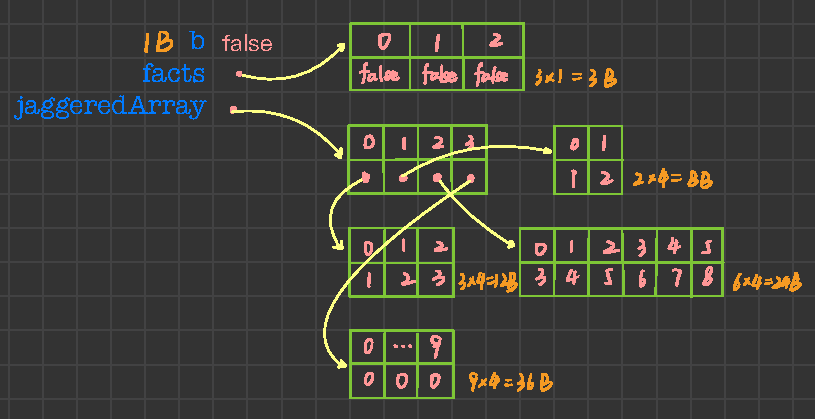
\includegraphics{1/Draft_裁剪页面.pdf}
    \caption{Problem2}
\end{figure}


\section*{Other things}

\begin{itemize}
    \item The figure style in problem2 refers to \href{https://cscircles.cemc.uwaterloo.ca/java_visualize/#}{Java Visualizer}.
    \item \LaTeX \space code refer to these things and was complied on texlive2020.
    \begin{itemize}
        \item  \href{https://www.eecs70.org/assets/misc/homework_template.tex}{UCB-CS70's given homework template.} 
        \item  \href{https://www.latexlive.com}{A free website useful to edit \LaTeX \space formula code.}
    \end{itemize}
    \item The purpose of writing in English is to adapt to bilingual teaching and to improve my poor English 
        writing skills in preparation for a possible future exchange program. 
\end{itemize}

\textbf{Thanks for your correcting and grading :).}

\end{document}

 
